\documentclass[10pt]{beamer}
\usepackage[utf8]{inputenc}

\usepackage{multirow,rotating}
\usepackage{color}
\usepackage{hyperref}
\usepackage{tikz-cd}
\usepackage{array}
\usepackage{siunitx}
\usepackage{mathtools,nccmath}%
\usepackage{etoolbox, xparse} 
\usetheme{CambridgeUS}
\usecolortheme{dolphin}
\usepackage{listings}

% set colors
\definecolor{myNewColorA}{RGB}{158, 27,50}
\definecolor{myNewColorB}{RGB}{158, 27,50}
\definecolor{myNewColorC}{RGB}{158, 27,50} % {130,138,143}
\setbeamercolor*{palette primary}{bg=myNewColorC}
\setbeamercolor*{palette secondary}{bg=myNewColorB, fg = white}
\setbeamercolor*{palette tertiary}{bg=myNewColorA, fg = white}
\setbeamercolor*{titlelike}{fg=myNewColorA}
\setbeamercolor*{title}{bg=myNewColorA, fg = white}
\setbeamercolor*{item}{fg=myNewColorA}
\setbeamercolor*{caption name}{fg=myNewColorA}
\usefonttheme{professionalfonts}
\usepackage{natbib}
\usepackage{hyperref}


\definecolor{white}{rgb}{1.0, 1.0, 1.0}
\definecolor{codegray}{rgb}{0.5,0.5,0.5}
\definecolor{codepurple}{rgb}{0.58,0,0.82}
\definecolor{codegreen}{rgb}{0,0.6,0}
%------------------------------------------------------------
% \titlegraphic{
\includegraphics[height=0.75cm]{uni-logo.png}} 

% logo of my university


\titlegraphic{%

\includegraphics[width=2.1cm]{uni-logo.png}
}

\setbeamerfont{title}{size=\large}
\setbeamerfont{subtitle}{size=\small}
\setbeamerfont{author}{size=\small}
\setbeamerfont{date}{size=\footnotesize}
\setbeamerfont{institute}{size=\footnotesize}
\title[UNI]{Práctica Dirigida 1 - Ejercicios (2,8,12,18)}%title
%\subtitle{ }%%subtitle
%\author[Roll Tide]{Malvaceda Canales Carlos Daniel\inst{1} and Crimson Ride\inst{1}}%%authors
\author[]{Cipriano Arroyo Bruno\\Catalino Morales Breiner\\Huanca Contreras Henry \\Malvaceda Canales Carlos Daniel}%%authors


\institute[UNI]{Universidad Nacional de Ingeniería}
\date[\textcolor{white}{Análisis y Modelamiento Numérico, 2022}]
{
Septiembre 28, 2022}

%------------------------------------------------------------
%This block of commands puts the Tabla de Contenido at the 
%beginning of each section and highlights the current section:
%\AtBeginSection[]
%{
%  \begin{frame}
%    \frametitle{Contents}
%    \tableofcontents[currentsection]
%  \end{frame}
%}
\AtBeginSection[]{

  \begin{frame}
  \vfill
  \centering
  \begin{beamercolorbox}[sep=8pt,center,shadow=true,rounded=true]{title}
    \usebeamerfont{title}\insertsectionhead\par%
  \end{beamercolorbox}
  \vfill
  \end{frame}
}
% ------Contents below------
%------------------------------------------------------------

\begin{document}

%The next statement creates the title page.
\frame{\titlepage}
\begin{frame}
\frametitle{Outline}
\tableofcontents
\end{frame}


% consider removing it if it's too redundant
\AtBeginSection[]
{
  \begin{frame}
    \frametitle{Tabla de Contenido}
    \tableofcontents[currentsection]
  \end{frame}
}
%-----------------------------------------------------------
\section{Pregunta 2}
\begin{frame}{Parte I}
Sea la sucesión definida por:\\
\hspace{2cm} a_1=$\sqrt{2}$ \wedge \hspace{1cm} a_n=$\sqrt{2a_{n-1}}$\\
demuestre que \left\lbrace{a_n}\right\rbrace_{n=1}^\infty \\ 
es convergente y determine su límite.\\
Demostración por inducción\\
1) para n=1, $a_1=&\sqrt{2}&$ para n=2, $a_2=&\sqrt{2&\sqrt{2}&}&$ de donde &\sqrt{2}&<&\sqrt{2&\sqrt{2}&} \Longrightarrow a_1<a_2\\
2) Hipotesis inductiva para n=k; $a_k<a_{k+1}$ por demostrar que n=k+1; osea $a_{k+1}< a_{k+2}$ en efecto:\\
como $a_k<a_{k+1}$ \Longrightarrow $2a_k<2a_{k+1}$\Longrightarrow $&\sqrt{2a_k}&<&\sqrt{2a_{k+1}}&$ por lo tanto $a_{k+1}<a_{k+2}$ es una sucesión monotona.

\end{frame}


\begin{frame}{Parte II}
Demostraremos que es acotada donde $a_n<2$ $\forall n$ por inducción\\
1) para n=1, $a_1=&\sqrt{2}&<2$ \\
2) Hipotesis inductiva para n=k; $a_k<2$ por demostrar para n=k+1, osea $a_{k+1}<2$, como a_k<2\Longrightarrow 2a_k<4 \Longrightarrow $&\sqrt{2a_k}&<2$ por lo tanto $a_{k+1}<2$ la sucesion es acotada.

Entonces aplicando el teorema de weierstrass al ser la sucesión monotona y acotada podemos decir que la sucesion converge.

\end{frame}
\begin{frame}{Parte III}
$\lim_{n \to \infty}(a_n)=L$ y como $a_n=&\sqrt{2a_{n-1}}&$ elevando al cuadrado se tiene $a_n^2=2a_{n-1}$ tomando limites podemos escribir  $\lim_{n \to \infty}(a_n^2)=\lim_{n \to \infty}(2a_{n-1})$\\
osea L^2=2L \Longrightarrow $L_1=0$ o $L_2=2$ como $a_n>0$ entonces $\lim_{n \to \infty}(a_n)=2$
\end{frame}

%------------------------------------------


%------------------------------------------------------------
\section{Pregunta 8}

%\begin{table}
%\centering
%\begin{tabular}
%...
%\end{tabular}
%\end{table}



\topskip0pt

\vspace*{\fill}
\begin{frame}{Pregunta 8}

\begin{quote}

Sea la sucesión 
\begin{math}
\{x_n\}
\end{math}
definida por:
\[{x_n=0,25e^{-n},x_0=0,1}\] 

Determine los valores usando el método \(\Delta^2\) de Aitkenn.




\end{quote}


\end{frame}


\vspace*{\fill}
%


\topskip0pt
\vspace*{\fill}
El método de Aitken \(\Delta^2\) está basado en la hipótesis que la sucesión 
\(\{\widehat{p}_n\}_{n\in \mathbb N}\) definida por :

\begin{equation}
\widehat{p}_n = p_n - \dfrac{(p_{n+1}-p_{n})^2}{p_{n+2}-2p_{n+1}+p_n}
\end{equation}
converge mas rápido a \(p\) que la sucesión original \(\{p\}_{\in \mathbb N}\).

\vspace*{\fill}
%


\newpage
\topskip0pt
\vspace*{\fill}

Calculando el valor de convergencia de la sucesión
\begin{math}
\{x_n\} = 0,25e^{-n} , x_{0}=0,1
\end{math}

\begin{equation}
    \lim_{n\to\infty} \{x_n\} = 0,25e^{-n} = 0
\end{equation}
Hallando los primeros valores de la sucesion 
	\begin{block}{Título del bloque}
		Lorem ipsum dolor sit amet, consectetur adipiscing elit. Integer lectus nisl, ultricies in feugiat rutrum, porttitor sit amet augue.
	\end{block}

\begin{equation}
   \ x_0\ = 0,1
\end{equation}
\begin{equation}
   \ x_{1}\ = 0,25e^{-1} 
\end{equation}
\begin{equation}
   \ x_{2}\ = 0,25e^{-2} 
\end{equation}
\begin{equation}
   \widehat{x}_{0} = x_0 - \dfrac{(x_{1}-x_{0})^2}{x_{2}-2x_{1}+x_0}
\end{equation}





\vspace*{\fill}
%




\begin{figure}{}
    \centering
    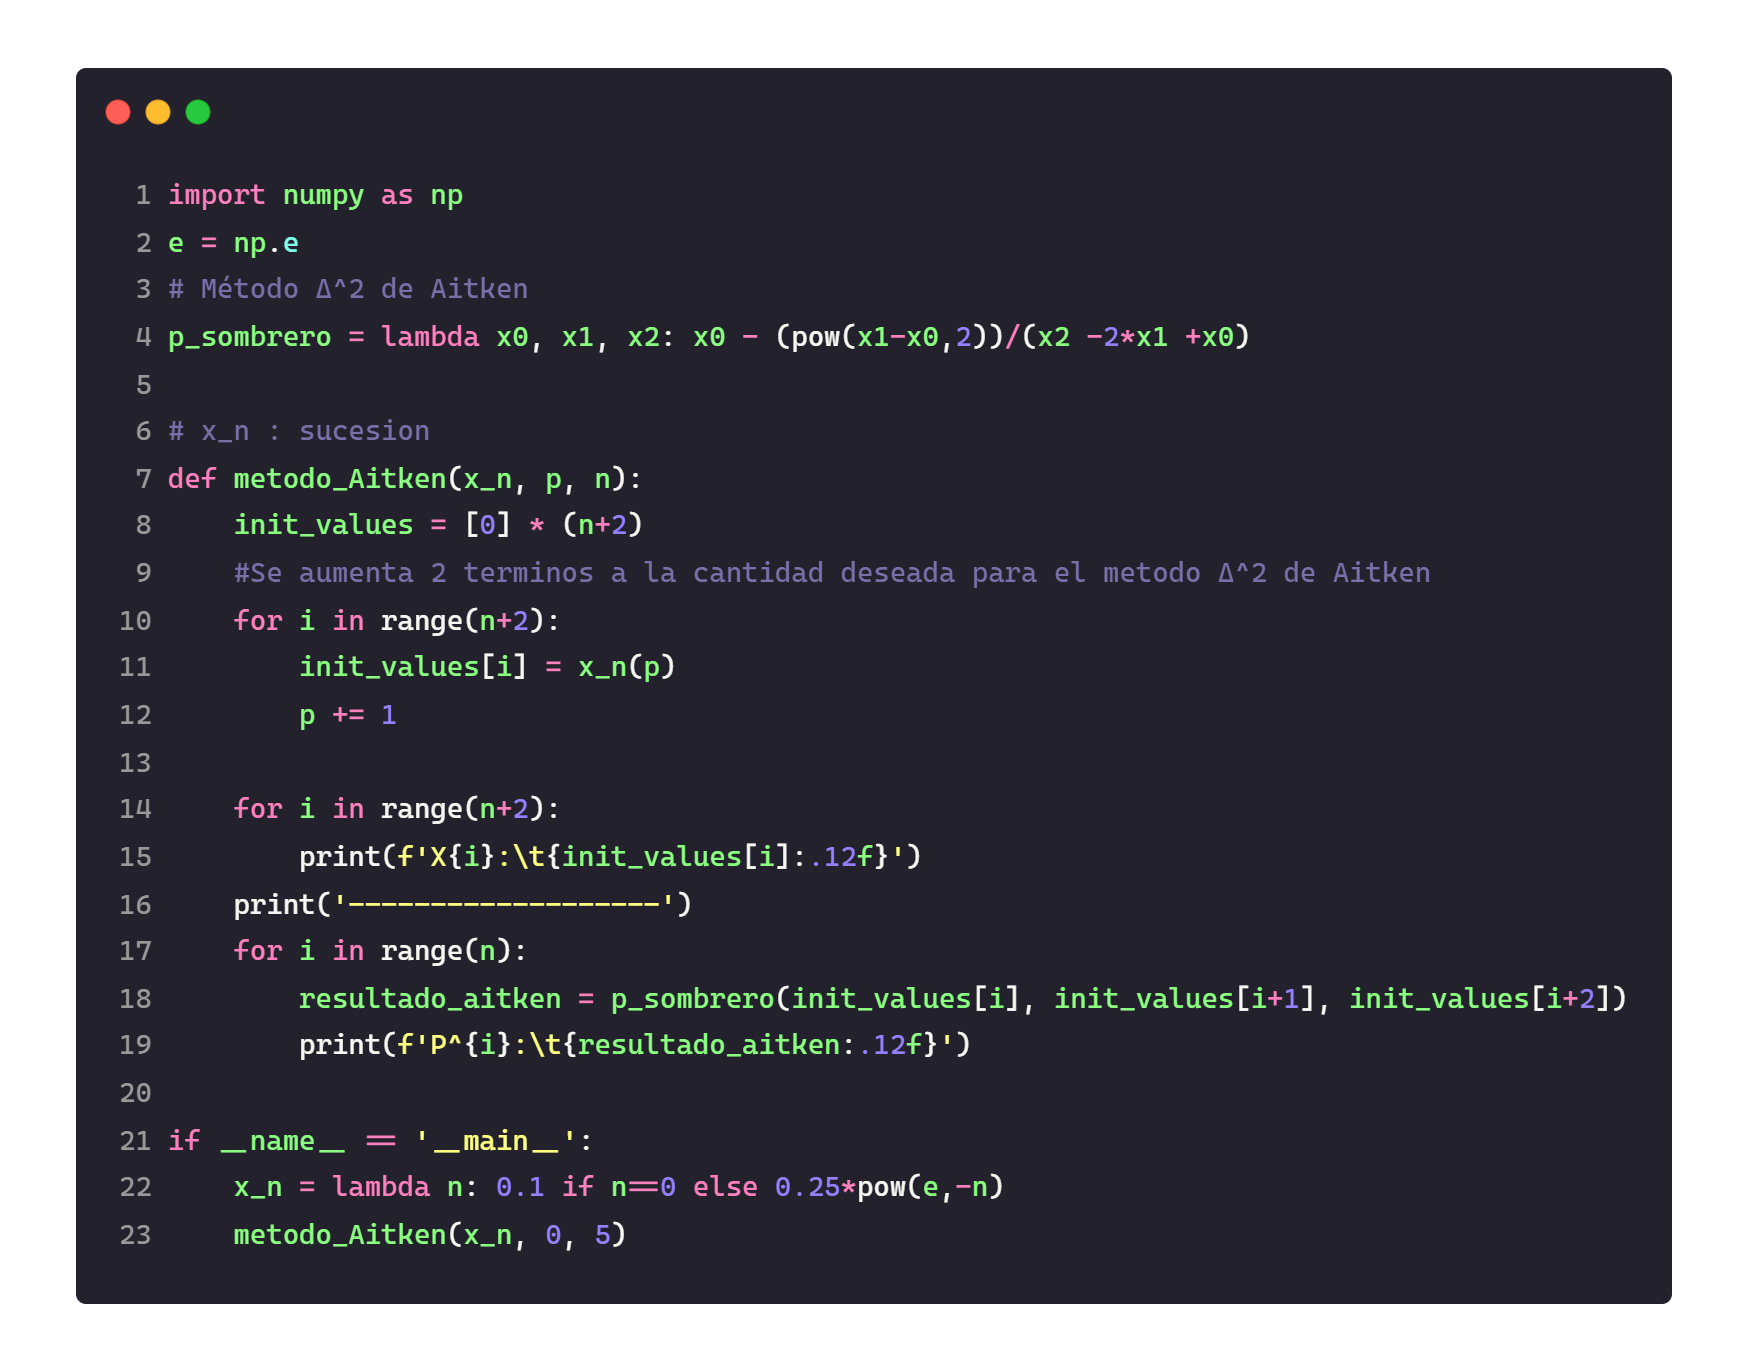
\includegraphics[width=11.5 cm]{pregunta8.png}
    \label{fig:Método Aitken}

\end{figure}

\newpage


\begin{table}
\centering

\topskip0pt
\vspace*{\fill}

\begin{tabular}{|c | c | c |} 

 \hline
 \({n}\) & \({x_n}\) & \widehat{p}_n  \\ [1ex] 
 \hline
 0 & 0.100000000000 & 0.101286937147  \\ 
 \hline
 1 & 0.091969860293 & 0.000000000000  \\
 \hline
 2 & 0.033833820809 & 0.000000000000  \\
 \hline
 3 & 0.012446767092 & 0.000000000000  \\
 \hline
 4 & 0.004578909722 & 0.000000000000  \\
 \hline
 5 & 0.001684486750 & 0.000000000000  \\
 \hline
 6 & 0.000619688044 & 0.000000000000  \\[1ex]
 \hline

\end{tabular}
 \caption{Sucesión generada por el método \(\Delta^2\) de Aitken}

\vspace*{\fill}
%

\end{table}




\section{Pregunta 12}
\lstdefinestyle{mystyle}{
  backgroundcolor=\color{white},
  commentstyle=\color{codegreen},
  keywordstyle=\color{magenta},
  numberstyle=\tiny\color{codegray},
  stringstyle=\color{codepurple},
  basicstyle=\ttfamily\large ,
  breakatwhitespace=false,         
  breaklines=true,                 
  captionpos=b,                    
  keepspaces=true,                 
  numbers=left,                    
  numbersep=5pt,                  
  showspaces=false,                
  showstringspaces=false,
  showtabs=false,                  
  tabsize=2
}

\lstset{style=mystyle}

\topskip0pt
\vspace*{\fill}
Implemente un programa en Python para convertir los siguientes números decimales a binarios con signo de 8 bits:\\ 
\centering
a) 56 \quad \quad \quad
b) 85 \\
c) 127 \quad \quad \quad
d) 27


\vspace*{\fill}
%

\newpage

\begin{figure}{}
    \centering
    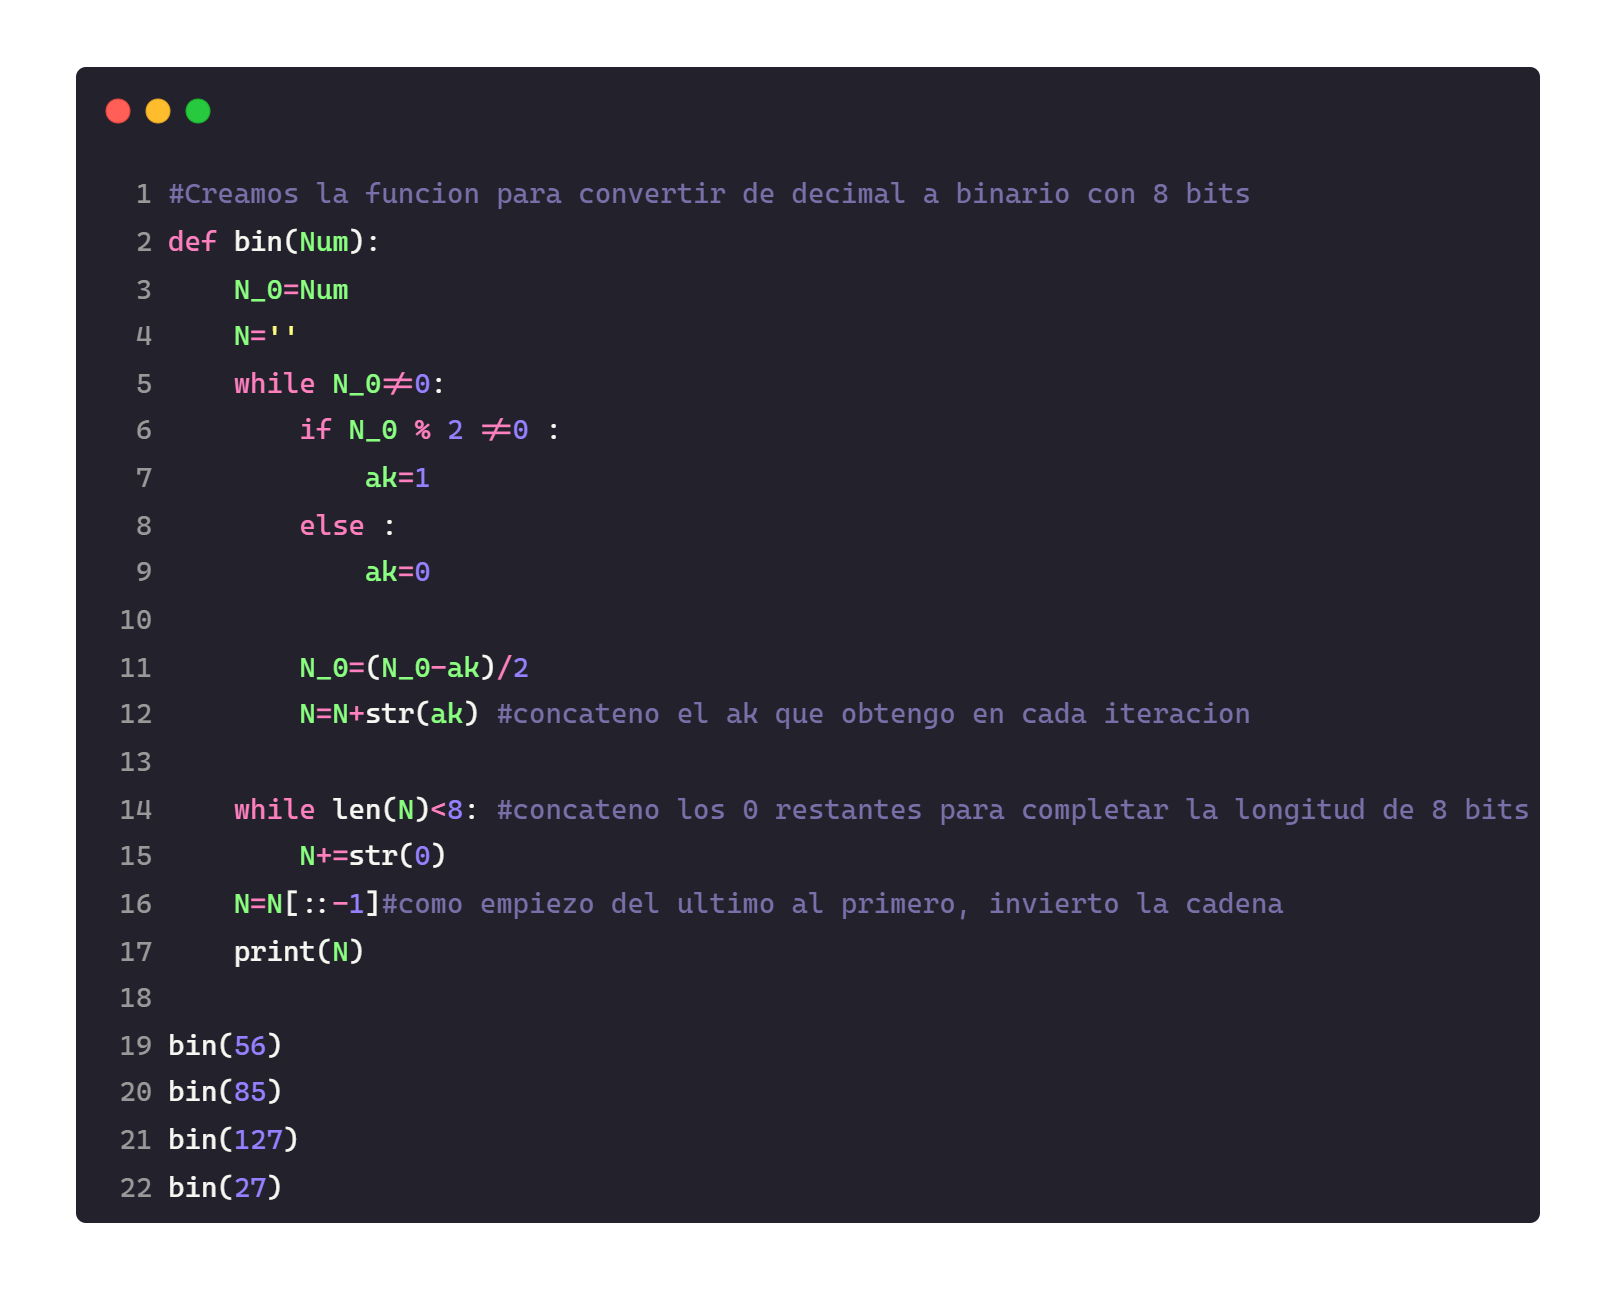
\includegraphics[width=11 cm]{pregunta12.png}
    %\caption{An image of a galaxy}
    \label{fig:Método Aitken}

\end{figure}

\newpage
\begin{table}

\topskip0pt
\vspace*{\fill}

\centering
\begin{tabular}{ | p{3cm} |p{3cm} | }

\hline
\multicolumn{2}{|c|}{Lista de Conversión} \\
\hline
Número & Conversion a 8 bits  \\
\hline
56 & 00111000  \\
85 & 01010101    \\
127 & 01111111  \\
27    & 00011011  \\
\hline
\end{tabular}
\caption{Numeros decimales y sus equivalentes en binario (8 bits) }


\vspace*{\fill}
%

\end{table}

%-------------------------------------------

\section{Pregunta 18}
\begin{frame}{Parte I}
Determinar el mayor, menor elemento positivo, número de elementos del conjunto $\mathbb{F}$(10,6,-9,9), asi como las siguientes operaciones x+y,x-y,xy,x/y, donde $x=\pi= 3.141592653589...$ e $y=\epsilon=2.7182818284590...$\\
De $\mathbb{F}$(10,6,-9,9) sabemos que B=10, t=6, L=-9, U=9\\
Además el conjunto $\mathbb{F}$ esta acotado de la forma:\\
x_{min}=B^{L-1}\leq |x| \leq B^U(1-B^{-t})=x_{max} \forall x \in \mathbb{F}\\
Por lo tanto el menor y mayor elemento positivo que puede tomar $\mathbb{F}$ seran:\\
$x_{min}=B^{L-1}=10^{-9-1}=10^{-10}$
$x_{max}=B^U(1-B^{-t}=10^9(1-10^{-6}=10^9-10^3=999999000$\\
El número de elementos de $\mathbb{F}$ esta dado por: 2(B-1)B^{t-1}(U-L+1)+1\\
\Longrightarrow \#elem=2(10-1)10^{6-1}(9-(-9)+1)+1\\
=2(9)*10^5*19+1\\
=342*10^5+1
=34200001
\end{frame}
\begin{frame}{Parte II}
$x=3.141592653589$\\
$y=2.7182818284590$\\
$fl(x)=0.314159*10$\\
$fl(y)=0.271828*10$\\
$i) x+y$ \hspace{5cm} $ii)x-y$\\
$fl(x)+fl(y)=0.585987*10$ \hspace{1.5cm}$fl(x)-fl(y)=0.042331*10$\\
$fl(fl(x)+fl(y))=0.585987*10$  \hspace{1cm}$fl(fl(x)-fl(y))=0.042331*10$\\
$iii) x.y$ \hspace{5cm} $iv)x/y$\\
$fl(x).fl(y)=0.085397212652*10^2$ \hspace{0.5cm} $fl(x)/fl(y)=1.15572715...*10$\\
$fl(fl(x).fl(y))=0.085397*10^2$ \hspace{1cm}$fl(fl(x)/fl(y))=0.115572*10$\\
\end{frame}



\end{document}



